\documentclass[border=10pt,margin=5pt,tikz,dvisvgm,rgb,utf8]{standalone}
\usepackage{ctex,xeCJK}  % 中文环境
\setCJKmainfont[BoldFont=Source Han Sans SC]{Source Han Serif SC}
\usepackage{calc,fontawesome,forest,smartdiagram,xcolor}
\usetikzlibrary{animations,arrows,automata,graphs,matrix,positioning,shadows,shapes}

\begin{document}
\renewcommand{\baselinestretch}{0.4}

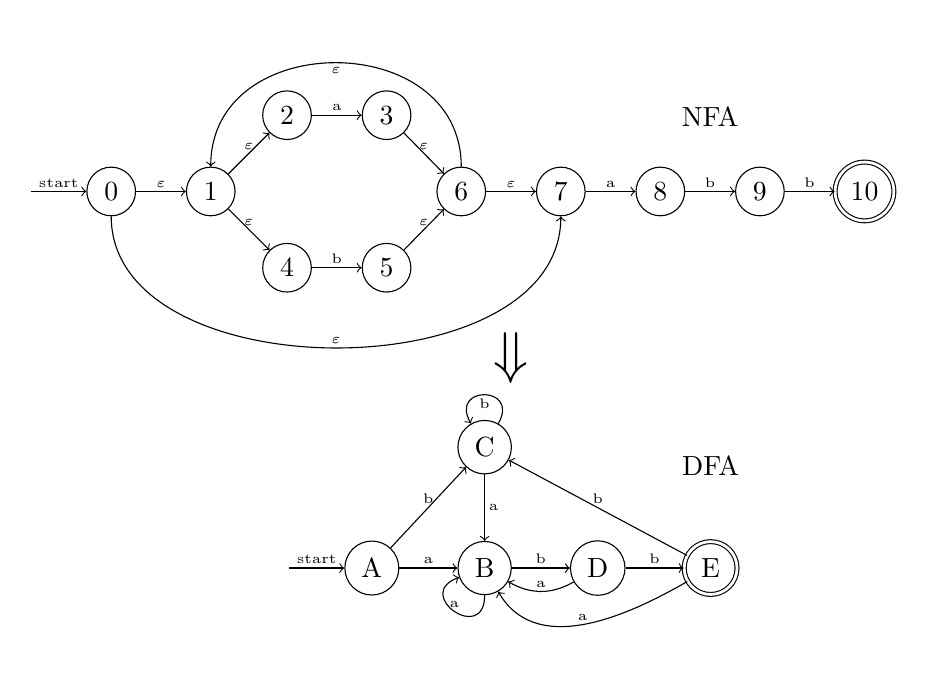
\begin{tikzpicture}
  % NFA
  \node[text width=-3em](NFAstart){};
  \node[circle, draw=black, right=2em of NFAstart](NFA0){0};
  \node[circle, draw=black, right=1.8em of NFA0](NFA1){1};
  \node[circle, draw=black, above right=2.1em of NFA1](NFA2){2};
  \node[circle, draw=black, below right=2.1em of NFA1](NFA4){4};
  \node[circle, draw=black, right=1.8em of NFA2](NFA3){3};
  \node[circle, draw=black, right=1.8em of NFA4](NFA5){5};
  \node[circle, draw=black, right=1.8em of $(NFA3)!0.5!(NFA5)$](NFA6){6};
  \node[circle, draw=black, right=1.8em of NFA6](NFA7){7};
  \node[circle, draw=black, right=1.8em of NFA7](NFA8){8};
  \node[circle, draw=black, right=1.8em of NFA8](NFA9){9};
  \node[circle, double, double distance=1pt, draw=black, right=1.8em of NFA9](NFA10){10};

  \node[above=2em of $(NFA8)!0.5!(NFA9)$](){NFA};

  \path[->]
  (NFAstart) edge node[above=-2pt]{\tiny start} (NFA0)
  (NFA0) edge node[above=-2pt]{\tiny $\varepsilon$} (NFA1)
  (NFA0) edge[out=270, in=270] node[above=-2pt]{\tiny $\varepsilon$} (NFA7)
  (NFA1) edge node[above=-2pt]{\tiny $\varepsilon$} (NFA2)
  (NFA1) edge node[above=-2pt]{\tiny $\varepsilon$} (NFA4)
  (NFA2) edge node[above=-2pt]{\tiny a} (NFA3)
  (NFA4) edge node[above=-2pt]{\tiny b} (NFA5)
  (NFA3) edge node[above=-2pt]{\tiny $\varepsilon$} (NFA6)
  (NFA5) edge node[above=-2pt]{\tiny $\varepsilon$} (NFA6)
  (NFA6) edge[out=90, in=90, min distance=5em] node[below=-2pt]{\tiny $\varepsilon$} (NFA1)
  (NFA6) edge node[above=-2pt]{\tiny $\varepsilon$} (NFA7)
  (NFA7) edge node[above=-2pt]{\tiny a} (NFA8)
  (NFA8) edge node[above=-2pt]{\tiny b} (NFA9)
  (NFA9) edge node[above=-2pt]{\tiny b} (NFA10);

  % transition
  \node[below=4.75em of $(NFA6)!0.5!(NFA7)$](){\huge $\Downarrow$};

  % DFA
  \node[text width=-3em, below=9.6em of NFA4](DFAstart){};
  \node[circle, draw=black, right=2em of DFAstart](DFAA){A};
  \node[circle, draw=black, right=2.1em of DFAA](DFAB){B};
  \node[circle, draw=black, above=2.4em of DFAB](DFAC){C};
  \node[circle, draw=black, right=2.1em of DFAB](DFAD){D};
  \node[circle, double, double distance=1pt, draw=black, right=2.1em of DFAD](DFAE){E};

  \node[above=2em of DFAE](){DFA};

  \path[->]
  (DFAstart) edge node[above=-2pt]{\tiny start} (DFAA)
  (DFAA) edge node[above=-2pt]{\tiny a} (DFAB)
  (DFAA) edge node[above=-2pt]{\tiny b} (DFAC)
  (DFAB) edge[out=270, in=200, min distance=1.8em] node[above=-2pt]{\tiny a} (DFAB)
  (DFAB) edge node[above=-2pt]{\tiny b} (DFAD)
  (DFAC) edge node[right=-2pt]{\tiny a} (DFAB)
  (DFAC) edge[out=60, in=120, min distance=1.6em] node[below=-2pt]{\tiny b} (DFAC)
  (DFAD) edge[out=210, in=330] node[above=-2pt]{\tiny a} (DFAB)
  (DFAD) edge node[above=-2pt]{\tiny b} (DFAE)
  (DFAE) edge[out=210, in=300] node[above=-2pt]{\tiny a} (DFAB)
  (DFAE) edge node[above=-2pt]{\tiny b} (DFAC);
\end{tikzpicture}

\end{document}
